\documentclass[a4paper,12pt]{article} % тип документа

%  Русский язык
\usepackage[T2A]{fontenc}			% кодировка
\usepackage[utf8]{inputenc}			% кодировка исходного текста
\usepackage[english,russian]{babel}	% локализация и переносы

\usepackage{graphicx}               % импорт изображений
\usepackage{wrapfig}                % обтекаемые изображения
\graphicspath{{pictures/}}          % обращение к подкаталогу с изображениями
\usepackage[14pt]{extsizes}         % для того чтобы задать нестандартный 14-ый размер шрифта
\usepackage{amsfonts}               % буквы с двойными штрихами
\usepackage[warn]{mathtext}         % русский язык в формулах
\usepackage{indentfirst}            % indent first
\usepackage[margin = 25mm]{geometry}% отступы полей
\usepackage{amsmath}                % можно выводить фигурные скобочки -- делать системы уравнений
\usepackage[table,xcdraw]{xcolor}   % таблицы
\usepackage{amsmath,amsfonts,amssymb,amsthm,mathtools} % Математика
\usepackage{wasysym}                % ???
\usepackage{upgreek}                % ???  
\usepackage{caption}
\usepackage{multirow}
\captionsetup{labelsep=period}
\usepackage{gensymb} % degree symbol


\begin{document}
	
	
	\begin{center}
		
		
		\textbf{НАЦИОНАЛЬНЫЙ ИССЛЕДОВАТЕЛЬСКИЙ УНИВЕРСИТЕТ \\ <<МОСКОВСКИЙ ФИЗИКО-ТЕХНИЧЕСКИЙ ИНСТИТУТ>>}
		\vspace{13ex}
		
		\textbf{Лабораторная работа 4.3.4\\ <<Преобразование Фурье в оптике>>}
		\vspace{40ex}
		
		\normalsize{Овсянников Михаил Александрович \\ студент группы Б01-001\\ 2 курс ФРКТ\\}
	\end{center}
	
	\vfill 
	
	\begin{center}
		г. Долгопрудный\\ 
		2022 г.
	\end{center}
	
	
	\thispagestyle{empty} % выключаем отображение номера для этой страницы
	\newpage
	
	\textbf{Цель работы:} пронаблюдать преобразование Фурье линзой, исследовать его свойства.
	
	\textbf{В работе используются:} гелий-неоновый лазер, кассета с набором сеток разного периода, щель с микрометрическим винтом, линзы, экран, линейка. 
	
	\section*{Теоретические сведения}
	Анализ сложного волнового поля во многих случаях целесообразно проводить, разлагая его на простейшие составляющие, например, представляя его в виде разложения по плоским волнам. При этом оказывается, что если мы рассматриваем поле, полученное после прохождения плоской монохроматической волны через предмет или транспарант (изображение предмета на фотоплёнке или стеклянной пластинке) с функцией пропускания $t(x)$, то разложение по плоским волнам соответствует преобразованию Фурье от этой функции. Если за предметом поставить линзу, то каждая плоская волна сфокусируется в свою точку в задней фокальной плоскости линзы. Таким образом, картина, наблюдаемая в фокальной плоскости линзы, даёт нам представление о спектре плоских волн падающего на линзу волнового поля. Поэтому можно утверждать, что с помощью линзы в оптике осуществляется пространственное преобразование Фурье.
	
	В данной работе и предполагается пронаблюдать это преобразование и изучить его свойства.
	
	\section*{Экспериментальная установка}
	Схема экспериментальной установки изображена на рисунке 1.
	
	\begin{figure}[h!]
		\centering
		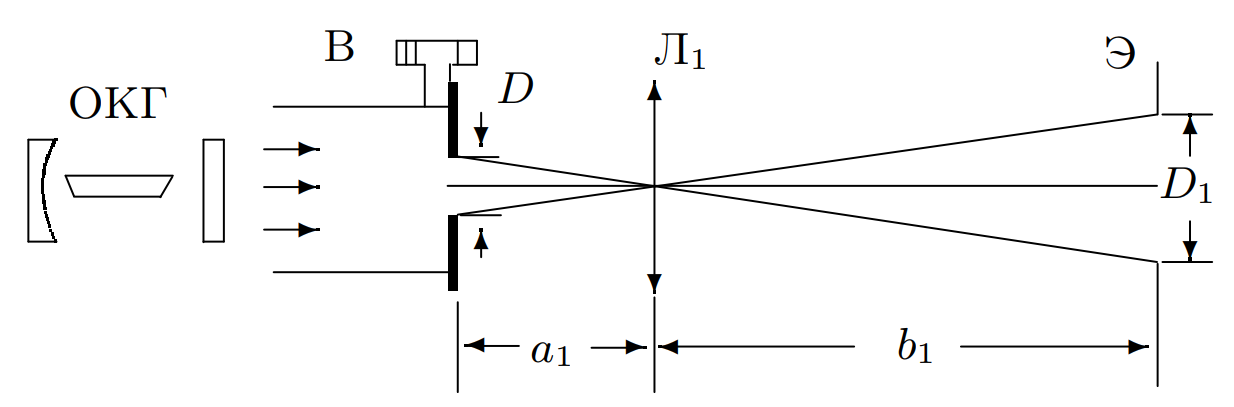
\includegraphics[scale=0.6]{Pictures/Установка}
		\caption{Экспериментальная установка}
	\end{figure}

	Щель переменной ширины $D$, снабжённая микрометрическим винтом В, освещается параллельным пучком света, излучаемым He-Ne лазером (радиус кривизны фронта волны велик по сравнению с фокусными расстояниями используемых в схеме линз). 
	
	Увеличенное изображение щели с помощью линзы Л$_1$ проецируется на экран Э. Величина изображения $D_1$ зависит от расстояний от линзы до предмета — $a_1$ и до изображения — $b_1$, т. е. от увеличения $\Gamma$ системы:
	
	\begin{equation*}
		\Gamma = \frac{D_1}{D} = \frac{b_1}{a_1}.
	\end{equation*}
	
	Изображение спектра щели образуется в задней фокальной плоскости $\Phi$ линзы Л$_1$. Размещая в плоскости $\Phi$ двумерные решётки-сетки, можно влиять на первичное изображение и получать мультиплицированное изображение щели. 
	
	Убрав линзу, можно наблюдать на экране спектр щели, а если заменить щель решёткой — спектр решётки. Крупные решётки дают на экране очень мелкую картину спектра, которую трудно промерить. В этом случае используют две линзы: первая (длиннофокусная) формирует первичное изображение — спектр, вторая (короткофокусная) — проецирует на экран увеличенное изображение спектра.
	
	\subsection*{А. Определение ширины щели}
		\begin{center}
			I. Определение ширины щели с помощью линзы
		\end{center}
	
	Установим тубус со щелью вплотную к выходному окну лазера. С помощью короткофокусной линзы Л$_1$ ($F_1 = 38$ мм) получим на экране Э увеличенное изображение щели.
	
	Меняя ширину щели от 50 до 500 мкм, снимем зависимость размера изображения $D_1$ от ширины щели $D$. Данные занесем в таблицу 1:
	
	\begin{table}[h!]
		\centering
		\begin{tabular}{|c|c|c|c|c|c|c|c|c|c|c|}
			\hline
			$D$, мкм  & 50 & 100 & 150 & 200 & 250 & 300 & 350 & 400 & 450  & 500  \\ \hline
			$D_1$, мм & 1,5  & 3,5 & 5   & 6   & 8   & 9,5   & 10,5   & 12  & 14,5 & 15,5 \\ \hline
		\end{tabular}
	\caption{Зависимость $D_1$ от $D$}
	\end{table}

	Измерим расстояния $a_1$ и $b_1$ для определения увеличения $\Gamma$ системы: $a_1 = (43 \pm 1)$ мм, $b_1 = (1318 \pm 1)$ мм. Также измерим расстояние от щели до экрана $L = a_1 + b_1 = 1361$ мм. Тогда увеличение системы можно найти как $\Gamma = \frac{b_1}{a_1} \approx 30,7$. 
	
	\begin{equation*}
		\sigma_\Gamma = \Gamma\sqrt{\left(\frac{\sigma_{a_1}}{a_1}\right)^2 + \left(\frac{\sigma_{b_1}}{b_1}\right)^2} = 0,7.
	\end{equation*}
	Тогда $\Gamma = (30,7 \pm 0,7)$.
	
	Но также можно его найти из данного соотношения:
	
	\begin{equation*}
		\frac{1}{a_1} + \frac{1}{b_1} = \frac{1}{F_1}
	\end{equation*}

	Учитывая, что $L = a_1 + b_1$, то $\frac{L}{F_1} = \left(a_1 + b_1\right)\left(\frac{1}{a_1} + \frac{1}{b_1}\right) = 2 + \Gamma + \frac{1}{\Gamma}$. Откуда получаем $\Gamma \approx 33,8$.
	В этом случае $\sigma_\Gamma \approx \sigma_{\frac{L}{F_1}} = \frac{\sigma_L}{F_1} = 0,04$.
	
	\noindent То есть $\Gamma = (33,80 \pm 0,04)$.
	
	Как видно, оба этих результата достаточно близки друг к другу, и в общем $\Gamma = (32,3 \pm 0,8)$.
	
	Зная увеличение линзы и размер изображения, рассчитаем ширину входной щели $D_{\text{л}}$:
	
	\begin{equation*}
		D_{\text{л}} = \frac{D_1}{\Gamma}
	\end{equation*}
	
	\begin{table}[h!]
		\centering
		\begin{tabular}{|c|c|c|c|c|c|c|c|c|c|c|}
			\hline
			$D$, мкм                                 & 50  & 100 & 150 & 200 & 250 & 300 & 350  & 400 & 450  & 500  \\ \hline
			$D_1$, мм                                & 1,5 & 3,5 & 5   & 6   & 8   & 9,5 & 10,5 & 12  & 14,5 & 15,5 \\ \hline
			$D_{\text{л}} = \frac{D_1}{\Gamma}$, мкм & 46  & 108 & 155 & 186 & 248 & 294 & 325  & 372 & 449  & 480  \\ \hline
		\end{tabular}
	\caption{}
	\end{table}
	
	Во всех случаях погрешность $\sigma_{D_{\text{л}}} = D_{\text{л}}\sqrt{\left(\frac{\sigma_{D_1}}{D_1}\right)^2 + \left(\frac{\sigma_{\Gamma}}{\Gamma}\right)^2}$.
	
	Например, для последнего эксперимента $\sigma_{D_{\text{л}}} = 33$ мкм.
	
	Как видим, расчетное и измеренное значения $D$ достаточно близки друг к другу во всех экспериментах.
	
	\vspace{35mm}
	\begin{center}	
	II. Определение ширины щели по её спектру
	\end{center}
	Получим на экране спектр щели (рисунок 2). Измерим ширину спектра для самой маленькой щели. Для большей точности будем измерять расстояние $X$ между удалёнными от центра минимумами, расположенными симметрично относительно центра картины, и отмечать порядок минимума $m$.
	
	\newpage
	\begin{figure}[h!]
		\centering
		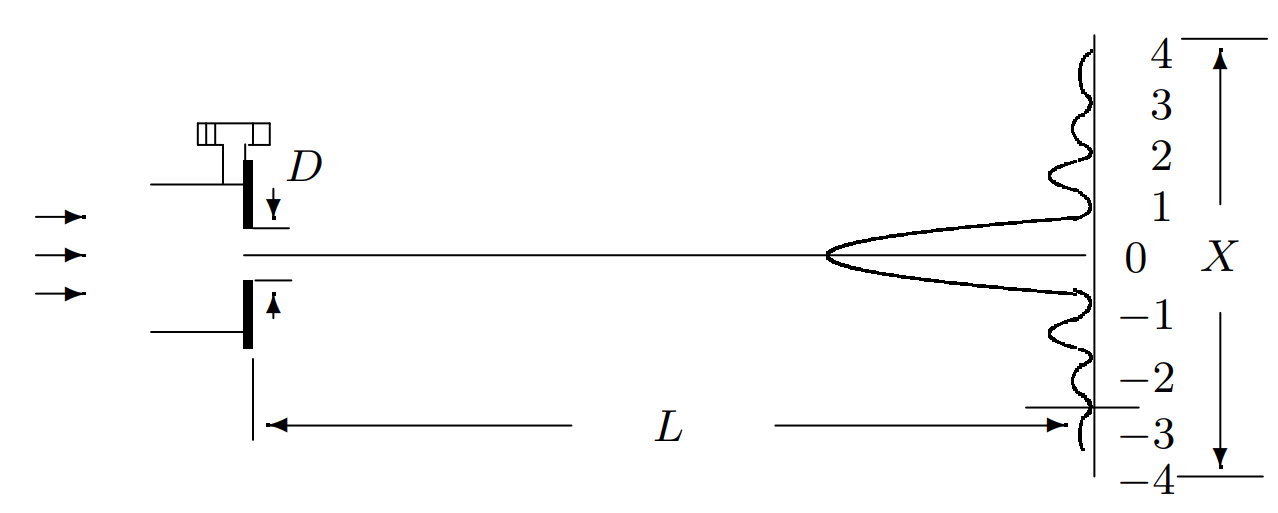
\includegraphics[scale=0.5]{Pictures/Спектр}
		\caption{Схема для определения ширины щели по спектру}
	\end{figure}
	
	
	Проведём серию измерений $X(m)$, меняя ширину щели в пределах от 50 мкм до 500 мкм. Результаты занесем в таблицу 3.
	
	\begin{table}[h!]
		\centering
		\begin{tabular}{|c|cc|c|}
			\hline
			$D$, мкм & \multicolumn{2}{c|}{$X(m)$, мм}                & $\left\langle \frac{X}{2m} \right\rangle$, мм \\ \hline
			50       & \multicolumn{1}{c|}{$X(1) = 33$} & $X(2) = 68$ & 16,8                                          \\ \hline
			100      & \multicolumn{1}{c|}{$X(1) = 17$} & $X(2) = 33$ & 8,4                                           \\ \hline
			150      & \multicolumn{1}{c|}{$X(1) = 11$} & $X(2) = 27$ & 6,1                                           \\ \hline
			200      & \multicolumn{1}{c|}{$X(1) = 8$}  & $X(2) = 17$ & 4,1                                           \\ \hline
			250      & \multicolumn{1}{c|}{$X(1) = 6$}  & $X(2) = 12$ & 3,0                                           \\ \hline
			300      & \multicolumn{1}{c|}{$X(1) = 5$}  & $X(2) = 10$ & 2,5                                           \\ \hline
			350      & \multicolumn{1}{c|}{$X(3) = 15$} & $X(4) = 18$ & 2,4                                           \\ \hline
			400      & \multicolumn{1}{c|}{$X(5) = 22$} & $X(8) = 34$ & 2,2                                           \\ \hline
			450      & \multicolumn{1}{c|}{$X(5) = 18$} & $X(8) = 29$ & 1,8                                           \\ \hline
			500      & \multicolumn{1}{c|}{$X(5) = 16$} & $X(8) = 26$ & 1,6                                           \\ \hline
		\end{tabular}
	\caption{Ширина спектра щели}
	\end{table}

	Расстояние от щели до экрана $L = 1318$ мм, длина волны лазера $\lambda = 632,8$ нм.
	
	По результатам измерений спектра рассчитаем ширину щели $D_c$:
	\begin{equation*}
		D_c = \dfrac{\lambda L}{\frac{X}{2m}}.
	\end{equation*}

	Результаты запишем в таблицу 4.
	
	Везде относительные погрешности $\delta_{D_c}^2 = \delta_X^2 + \delta_L^2$.
	
	\newpage
	
	\begin{table}[h!]
		\centering
		\begin{tabular}{|c|c|c|c|c|c|c|c|c|c|c|}
			\hline
			$D$, мкм            & 50 & 100 & 150 & 200 & 250 & 300 & 350 & 400 & 450 & 500 \\ \hline
			$D_c$, мкм          & 50 & 99  & 137 & 203 & 278 & 333 & 347 & 379 & 463 & 521 \\ \hline
			$\sigma_{D_c}$, мкм & 2  & 6   & 11  & 25  & 46  & 67  & 36  & 22  & 32  & 41  \\ \hline
		\end{tabular}
	\caption{Сравнение расчетного и измеренного значений $D$}
	\end{table}

	Построим зависимости $D_{\text{л}} = f(D)$ и $D_c = f(D)$ на одном графике:
	
	\begin{figure}[h!]
		\centering
		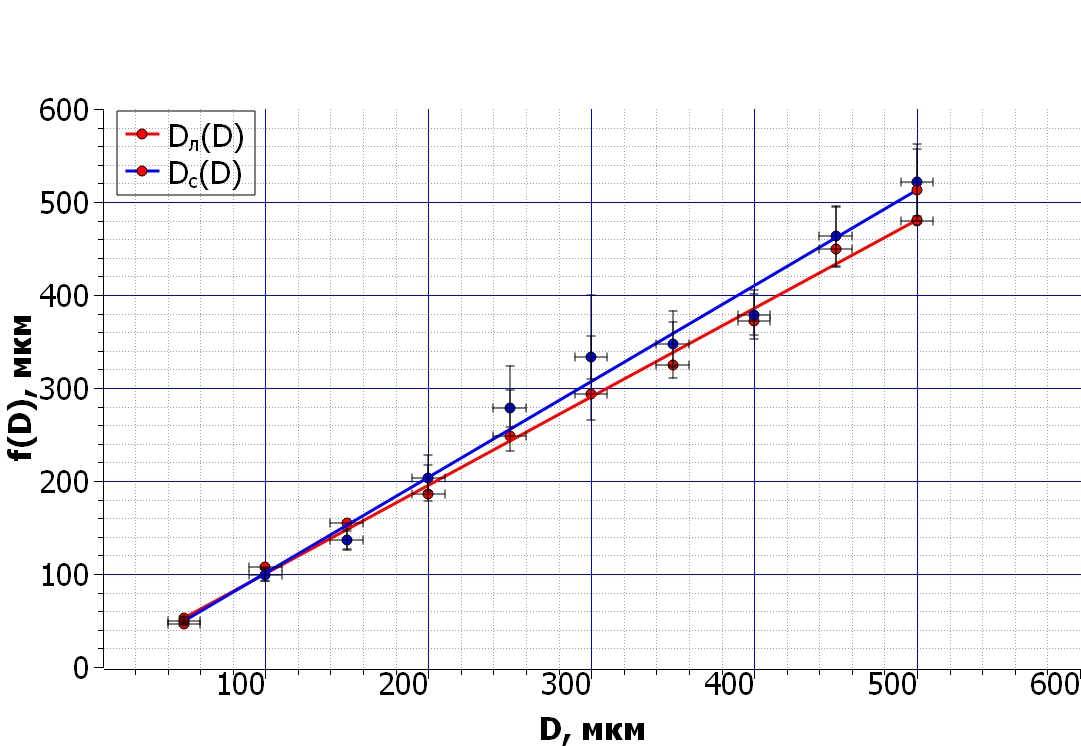
\includegraphics[scale=0.7]{Pictures/График}
		\caption{Сравнение полученных результатов}
	\end{figure}

	Видно, что результаты экспериментов достаточно близки друг к другу и в пределах погрешностей совпадают.
	
	
	\newpage
	
	Вот графики для $D_{\text{л}} = f(D)$ и $D_c = f(D)$ по отдельности, чтобы можно было проанализировать их лучше.
	
	\begin{figure}[h!]
		\centering
		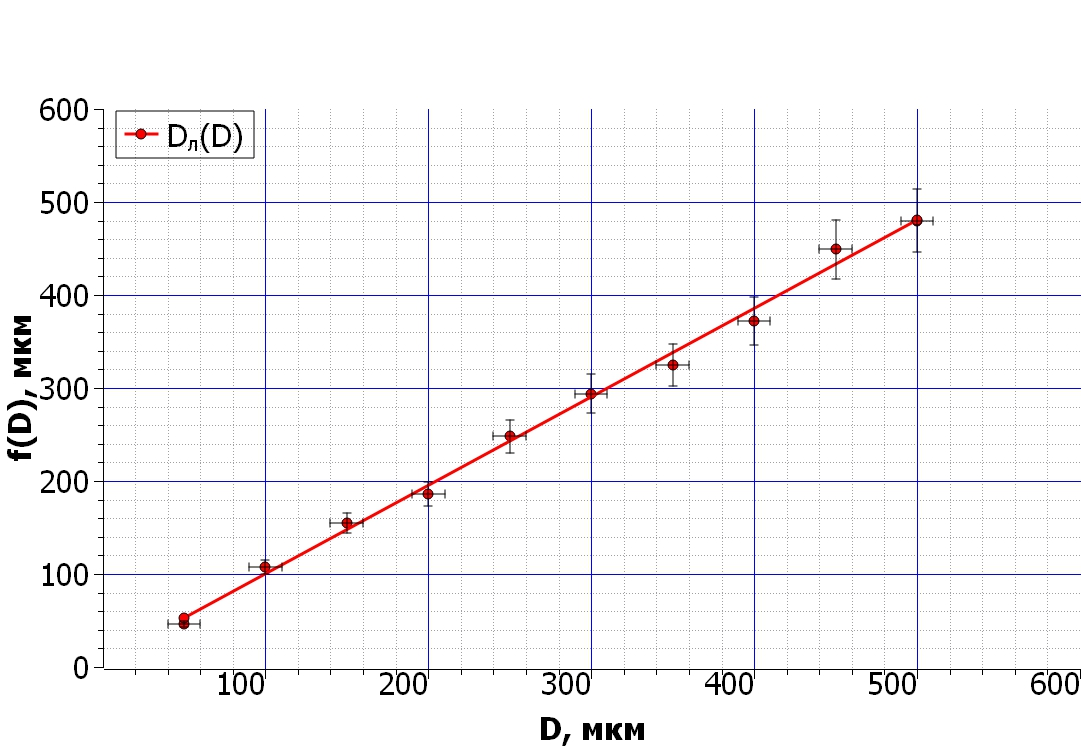
\includegraphics[scale=0.6]{Pictures/График_Линза}
		\caption{$D_{\text{л}} = f(D)$}
	\end{figure}
	
	\begin{figure}[h!]
		\centering
		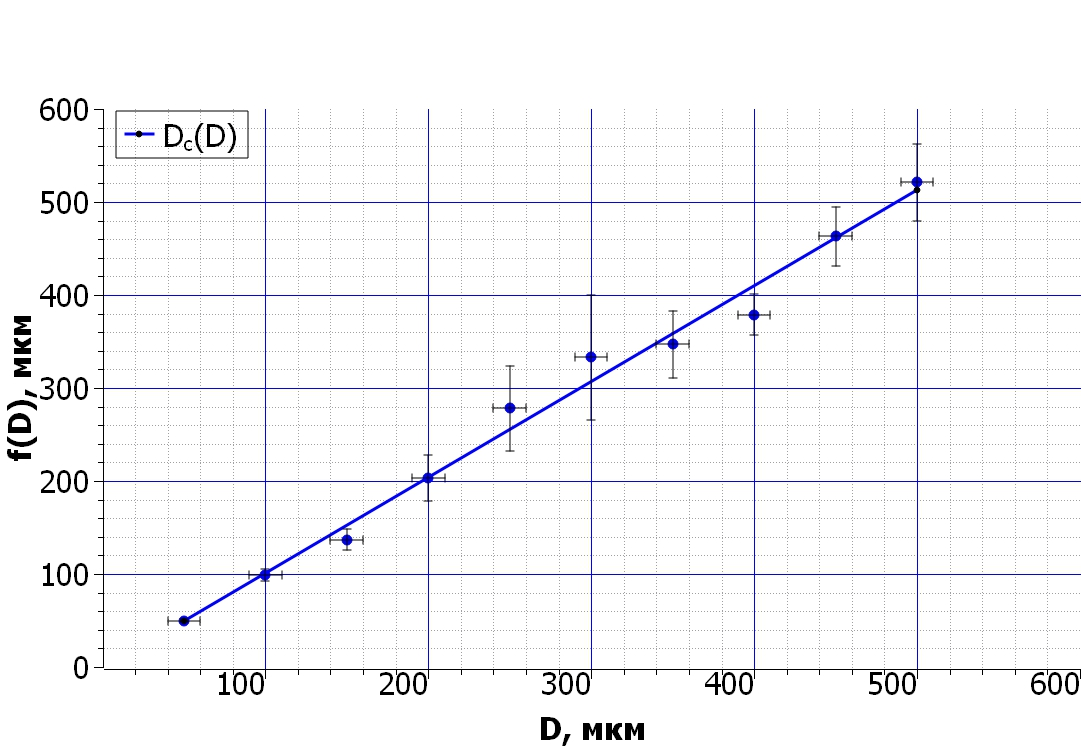
\includegraphics[scale=0.6]{Pictures/График_Спектр}
		\caption{$D_c = f(D)$}
	\end{figure}
	
	
	\subsection*{Б. Определение периода решёток}
	
	\begin{center}
			I. Определение периода по спектру на удалённом экране
	\end{center}
	
	Поставим кассету с двумерными решётками вплотную к выходному окну лазера. Измерим расстояние $L$ от кассеты до экрана: $L = 1343$ мм.
	 
	Для каждой сетки измерим расстояние $X$ между $m$-ми максимумами и отметим $m$ — порядок максимума и определим период каждой решётки $d_c$ = $f$(№), используя соотношение:
	\begin{equation*}
		d_c = \frac{\lambda L}{\frac{X}{2m}}.
	\end{equation*}
	
	\vspace{3mm}
	\textbf{{\large\textit{Сетка №1:}}}
	\begin{table}[h!]
		\centering
		\begin{tabular}{|c|c|}
			\hline
			$m$ & $X(m)$, мм \\ \hline
			1   & 62         \\ \hline
			2   & 126        \\ \hline
			3   & 211        \\ \hline
		\end{tabular}
	\caption{Сетка №1}
	\end{table}

	\begin{equation*}
		d_c = \frac{\lambda L}{\left\langle\frac{X}{2m}\right\rangle} = 26,2 \text{ мкм}. \hspace{15mm} \sigma_{d_c} = d_c\sqrt{\left(\frac{\sigma_L}{L}\right)^2 + \left(\frac{\sigma_X}{X}\right)^2} = 0,4 \text{ мкм}.
	\end{equation*}

	\begin{center}
		$\boxed{d_c = (26,2 \pm 0,4) \text{ мкм}}$
	\end{center}


	\vspace{3mm}
	\textbf{{\large\textit{Сетка №2:}}}
	\begin{table}[h!]
		\centering
		\begin{tabular}{|c|c|}
			\hline
			$m$ & $X(m)$, мм \\ \hline
			1   & 49         \\ \hline
			2   & 97        \\ \hline
			3   & 169        \\ \hline
		\end{tabular}
		\caption{Сетка №2}
	\end{table}
	
	\begin{equation*}
		d_c = \frac{\lambda L}{\left\langle\frac{X}{2m}\right\rangle} = 33,2 \text{ мкм}. \hspace{15mm} \sigma_{d_c} = d_c\sqrt{\left(\frac{\sigma_L}{L}\right)^2 + \left(\frac{\sigma_X}{X}\right)^2} = 0,7 \text{ мкм}.
	\end{equation*}
	
	\begin{center}
		$\boxed{d_c = (33,2 \pm 0,7) \text{ мкм}}$
	\end{center}


	\newpage
	\textbf{{\large\textit{Сетка №3:}}}
	\begin{table}[h!]
		\centering
		\begin{tabular}{|c|c|}
			\hline
			$m$ & $X(m)$, мм \\ \hline
			1   & 25         \\ \hline
			2   & 49        \\ \hline
			3   & 74        \\ \hline
		\end{tabular}
		\caption{Сетка №3}
	\end{table}
	
	\begin{equation*}
		d_c = \frac{\lambda L}{\left\langle\frac{X}{2m}\right\rangle} = 69 \text{ мкм}. \hspace{15mm} \sigma_{d_c} = d_c\sqrt{\left(\frac{\sigma_L}{L}\right)^2 + \left(\frac{\sigma_X}{X}\right)^2} = 3 \text{ мкм}.
	\end{equation*}
	
	\begin{center}
		$\boxed{d_c = (69 \pm 3) \text{ мкм}}$
	\end{center}


	\textbf{{\large\textit{Сетка №4:}}}
	\begin{table}[h!]
		\centering
		\begin{tabular}{|c|c|}
			\hline
			$m$ & $X(m)$, мм \\ \hline
			2   & 24         \\ \hline
			3   & 36        \\ \hline
			4   & 49        \\ \hline
		\end{tabular}
		\caption{Сетка №4}
	\end{table}
	
	\begin{equation*}
		d_c = \frac{\lambda L}{\left\langle\frac{X}{2m}\right\rangle} = 141 \text{ мкм}. \hspace{15mm} \sigma_{d_c} = d_c\sqrt{\left(\frac{\sigma_L}{L}\right)^2 + \left(\frac{\sigma_X}{X}\right)^2} = 6 \text{ мкм}.
	\end{equation*}
	
	\begin{center}
		$\boxed{d_c = (141 \pm 6) \text{ мкм}}$
	\end{center}

	\textbf{{\large\textit{Сетка №5:}}}
	\begin{table}[h!]
		\centering
		\begin{tabular}{|c|c|}
			\hline
			$m$ & $X(m)$, мм \\ \hline
			3   & 28         \\ \hline
			4   & 36        \\ \hline
			5   & 46        \\ \hline
		\end{tabular}
		\caption{Сетка №5}
	\end{table}
	
	\begin{equation*}
		d_c = \frac{\lambda L}{\left\langle\frac{X}{2m}\right\rangle} = 185 \text{ мкм}. \hspace{15mm} \sigma_{d_c} = d_c\sqrt{\left(\frac{\sigma_L}{L}\right)^2 + \left(\frac{\sigma_X}{X}\right)^2} = 7 \text{ мкм}.
	\end{equation*}
	
	\begin{center}
		$\boxed{d_c = (185 \pm 7) \text{ мкм}}$
	\end{center}

	\newpage
	Таким образом:
	
	\begin{table}[h!]
		\centering
		\begin{tabular}{|c|c|}
			\hline
			№ решетки & $d_c$, мкм     \\ \hline
			1         & $26,2 \pm 0,4$ \\ \hline
			2         & $33,2 \pm 0,7$ \\ \hline
			3         & $69 \pm 3$     \\ \hline
			4         & $141 \pm 6$    \\ \hline
			5         & $185 \pm 7$    \\ \hline
		\end{tabular}
	\caption{Общие результаты периодов решеток}
	\end{table}

	\vspace{15mm}
	\begin{center}
		II. Определение периода решёток по увеличенному изображению спектра
	\end{center}

	\begin{figure}[h!]
		\centering
		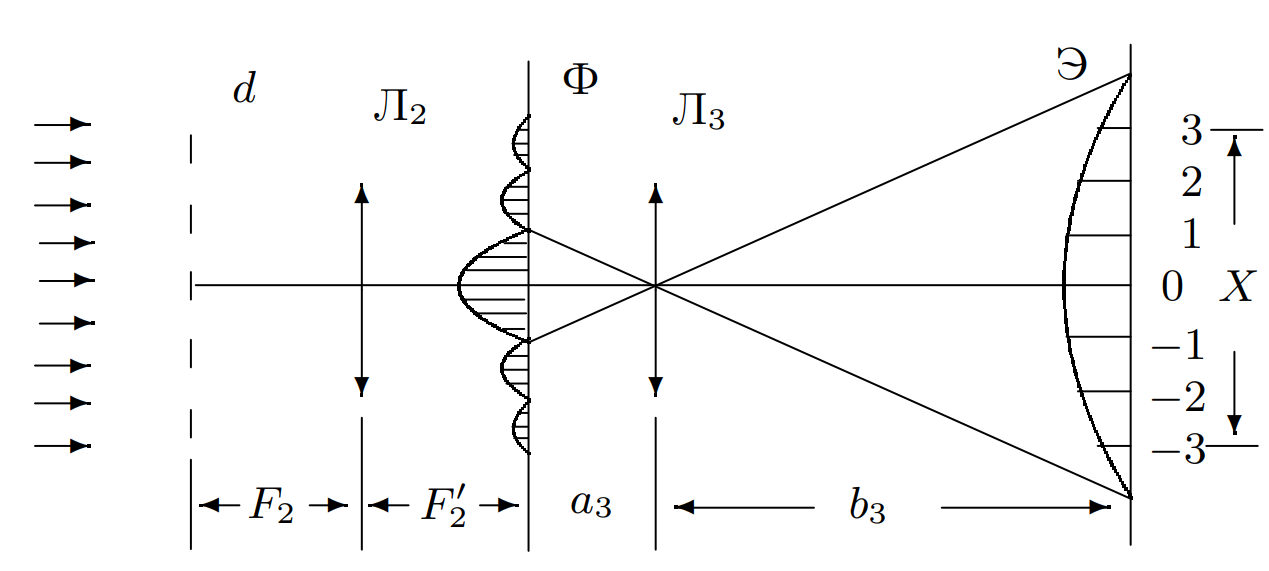
\includegraphics[scale=0.6]{Pictures/Схема2}
		\caption{Схема определения периода решётки по увеличенному изображению спектра}
	\end{figure}
	
	Линзу Л$_2$ с максимальным фокусом $F_2 = 110$ мм поставим на расстоянии $\thicksim F_2$ от кассеты. В плоскости $\Phi$ линза Л$_2$ даёт фурье-образ сетки — её спектр, а короткофокусная линза Л$_3$ с фокусом $F_3 = 25$ мм cоздаёт на экране увеличенное изображение этого спектра.
	
	Измерим расстояния $a_3$ и $b_3$: $a_3 = (30 \pm 1)$ мм, $b_3 = (1095 \pm 1)$ мм. Тогда увеличение линзы Л$_3: \Gamma_3 = \frac{b_3}{a_3}$. $\Gamma_3 = (37 \pm 1)$.
	
	Измерим $X$ и $m$ для всех сеток, где это возможно. Зная увеличение линзы Л$_3$, рассчитаем период сетки $d_{\text{л}}$:
	\begin{equation*}
		d_{\text{л}} = \frac{\lambda \Gamma_3 F_2}{\frac{X}{2m}}, \hspace{35mm} \sigma_{d_{\text{л}}} = d_{\text{л}}\sqrt{\left(\frac{\sigma_{\Gamma_3}}{\Gamma_3}\right)^2 + \left(\frac{\sigma_{X}}{X}\right)^2}.
	\end{equation*}


	\textbf{{\large\textit{Сетка №1:}}}
	\begin{table}[h!]
		\centering
		\begin{tabular}{|c|c|}
			\hline
			$m$ & $X(m)$, мм \\ \hline
			1   & 195         \\ \hline
		\end{tabular}
		\caption{Сетка №1}
	\end{table}

	\begin{center}
		$\boxed{d_{\text{л}} = (26,4 \pm 0,7) \text{ мкм}}$
	\end{center}

	\textbf{{\large\textit{Сетка №2:}}}
	\begin{table}[h!]
		\centering
		\begin{tabular}{|c|c|}
			\hline
			$m$ & $X(m)$, мм \\ \hline
			1   & 165         \\ \hline
		\end{tabular}
		\caption{Сетка №2}
	\end{table}
	
	\begin{center}
		$\boxed{d_{\text{л}} = (31,2 \pm 0,9) \text{ мкм}}$
	\end{center}

	\textbf{{\large\textit{Сетка №3:}}}
	\begin{table}[h!]
		\centering
		\begin{tabular}{|c|c|}
			\hline
			$m$ & $X(m)$, мм \\ \hline
			1   & 97         \\ \hline
			2   & 195        \\ \hline
		\end{tabular}
		\caption{Сетка №3}
	\end{table}
	
	\begin{center}
		$\boxed{d_{\text{л}} = (53 \pm 2) \text{ мкм}}$
	\end{center}

	\newpage
	\textbf{{\large\textit{Сетка №4:}}}
	\begin{table}[h!]
		\centering
		\begin{tabular}{|c|c|}
			\hline
			$m$ & $X(m)$, мм \\ \hline
			1   & 37         \\ \hline
			2   & 73         \\ \hline
			3   & 110        \\ \hline
		\end{tabular}
		\caption{Сетка №4}
	\end{table}
	
	\begin{center}
		$\boxed{d_{\text{л}} = (140 \pm 5) \text{ мкм}}$
	\end{center}

	\textbf{{\large\textit{Сетка №5:}}}
	\begin{table}[h!]
		\centering
		\begin{tabular}{|c|c|}
			\hline
			$m$ & $X(m)$, мм \\ \hline
			1   & 27         \\ \hline
			2   & 58         \\ \hline
			3   & 82        \\ \hline
		\end{tabular}
		\caption{Сетка №5}
	\end{table}
	
	\begin{center}
		$\boxed{d_{\text{л}} = (185 \pm 9) \text{ мкм}}$
	\end{center}


	Итого:
	
	\begin{table}[h!]
		\centering
		\begin{tabular}{|c|c|}
			\hline
			№ решетки & $d_{\text{л}}$, мкм     \\ \hline
			1         & $26,4 \pm 0,7$ \\ \hline
			2         & $31,2 \pm 0,9$ \\ \hline
			3         & $53 \pm 2$     \\ \hline
			4         & $140 \pm 5$    \\ \hline
			5         & $185 \pm 9$    \\ \hline
		\end{tabular}
		\caption{Общие результаты периодов решеток}
	\end{table}


	\newpage
	\subsection*{В. Мультиплицирование}
	\begin{figure}[h!]
		\centering
		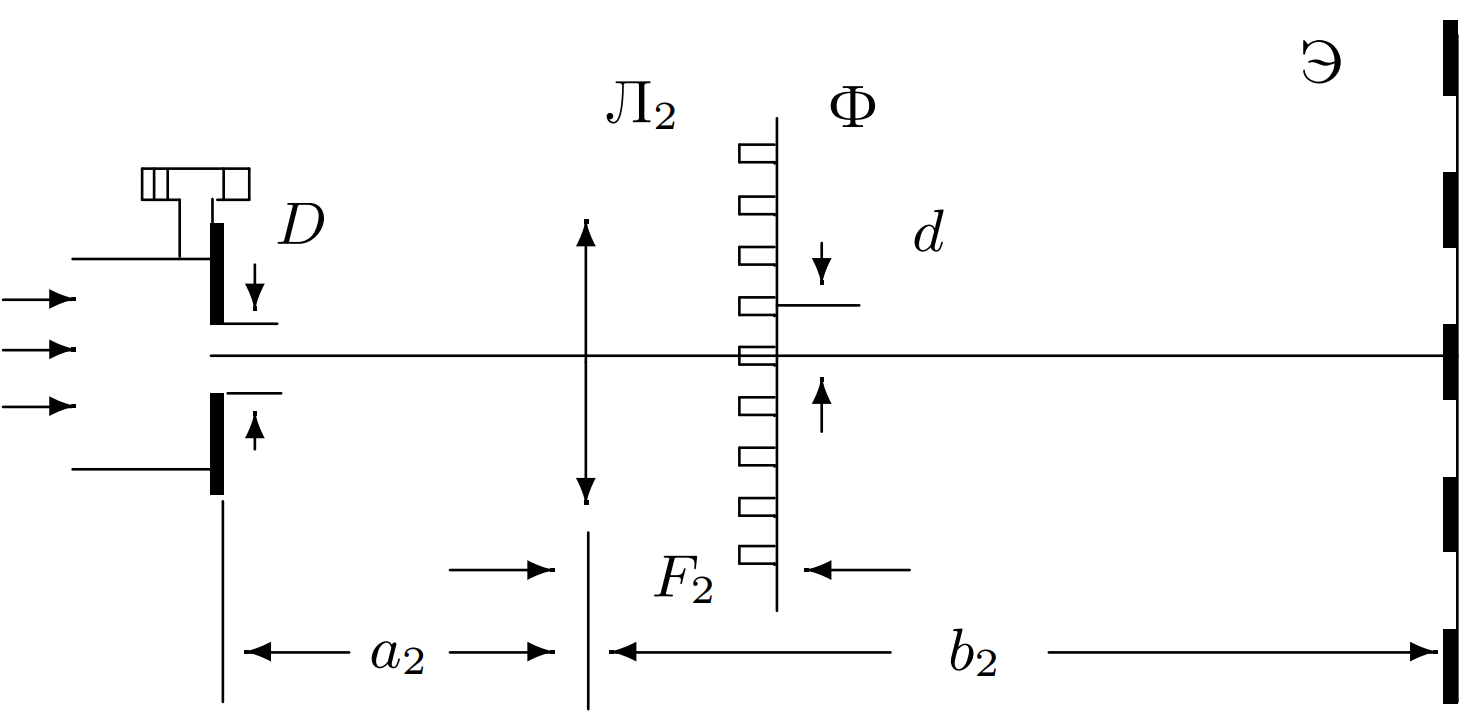
\includegraphics[scale=0.5]{Pictures/Мультиплицирование}
		\caption{Схема для наблюдения мультиплицирования}
	\end{figure}

	Снова поставим тубус со щелью к окну лазера и найдем на экране резкое изображение щели с помощью линзы Л$_2$. В фокальной плоскости $\Phi$ линзы Л$_2$ поставим кассету с сетками, которые будут «рассекать» фурье-образ щели — осуществлять пространственную фильтрацию. Подберем такую ширину входной щели $D$, чтобы на экране можно было наблюдать мультиплицированное изображение для всех сеток.
	
	Снимем зависимость $Y$ -- расстояние между удалёнными изображениями щели -- и $K$ -- число промежутков между изображениями -- от номера сетки для фиксированной ширины входной щели $D = 20$ мкм.
	
	Измерим расстояния $a_2$ и $b_2$ для расчёта увеличения второй линзы Г$_2$: $a_2 = (115 \pm 1)$ мм, $b_2 = (1230 \pm 1)$ мм. Тогда $\Gamma_2 = \frac{b_2}{a_2}$. $\Gamma_2 = (11,7 \pm 0,1)$.
	
	\begin{table}[h!]
		\centering
		\begin{tabular}{|c|c|c|}
			\hline
			№ сетки & $K$ & $Y$, мм \\ \hline
			1       & 4   & 112     \\ \hline
			2       & 6   & 93      \\ \hline
			3       & 8   & 76      \\ \hline
			4       & 10  & 48      \\ \hline
			5       & 12  & 43      \\ \hline
		\end{tabular}
	\caption{Зависимость $Y$ и $K$ от номера решетки}
	\end{table}
	
	\newpage

	Рассчитаем периоды $\Delta y$ «фиктивных» решёток, которые дали бы такую же периодичность на экране:
	\begin{equation*}
		\Delta y = \frac{Y}{K\Gamma_2}, \hspace{35mm} \sigma_{\Delta y} = \Delta y \sqrt{\left(\frac{\sigma_Y}{Y}\right)^2 + \left(\frac{\sigma_{\Gamma_2}}{\Gamma_2}\right)^2}.
	\end{equation*}

	\begin{table}[h!]
		\centering
		\begin{tabular}{|c|c|c|}
			\hline
			№ сетки & $\Delta y$, мм & $\sigma_{\Delta y}$, мм \\ \hline
			1       & 28,0           & 0,4                     \\ \hline
			2       & 15,5           & 0,2                     \\ \hline
			3       & 9,5            & 0,2                     \\ \hline
			4       & 4,8            & 0,1                     \\ \hline
			5       & 3,6            & 0,1                     \\ \hline
		\end{tabular}
	\caption{Зависимость $\Delta y$ от номера решетки}
	\end{table}

	Построим график зависимости $\Delta y = f(1/d_c)$:
	
	\begin{figure}[h!]
		\centering
		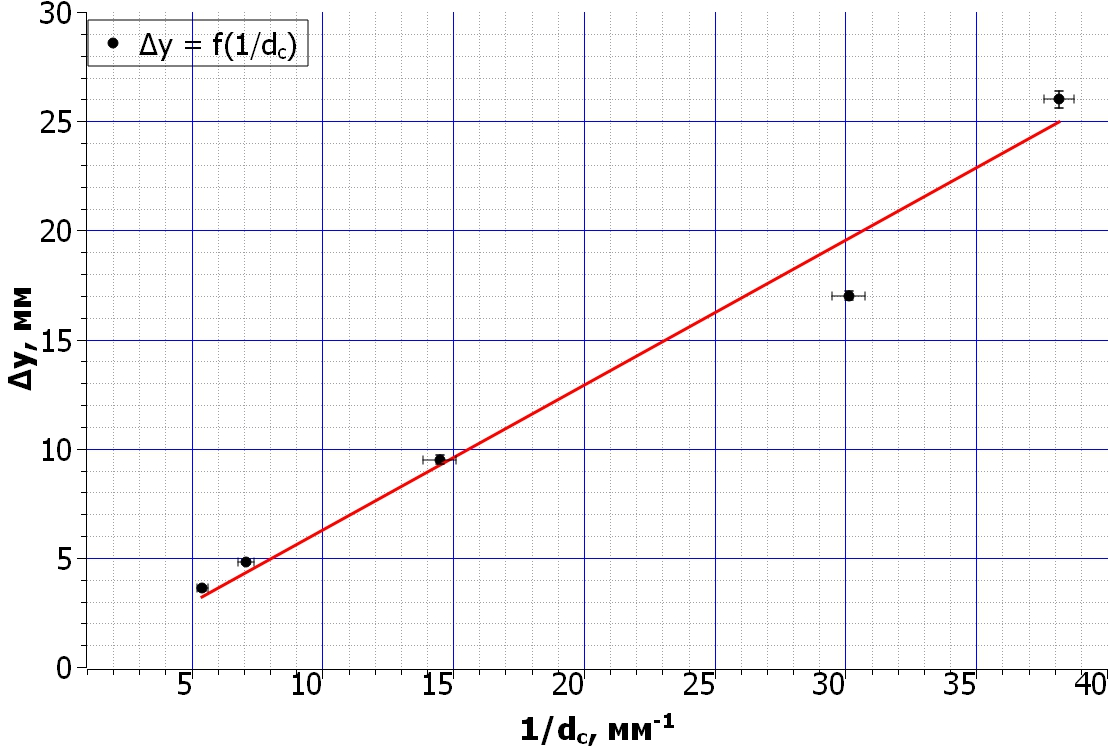
\includegraphics[scale=0.6]{Pictures/Dy}
		\caption{$\Delta y = f(1/d_c)$}
	\end{figure}

	Точки неплохо ложатся на прямую, как оно и должно быть теоретически, однако четвертая точка выбивается из этой тенденции, что связано с неточностью измерений.
	
	\newpage
	\subsection*{Г. Влияние щелевой диафрагмы на изображение сетки}
	
	\begin{figure}[h!]
		\centering
		
\includegraphics[scale=0.9]{Pictures/Изначальн}
		\caption{Изначальная картина сетки}
	\end{figure}
	
	Поставим на место щели кассету с сетками и сфокусируем на экран изображение сетки. Поставим в плоскости $\Phi$ вертикальную щель и проследим за изменением изображения на экране при сужении щели. 
	
	\begin{figure}[h!]
		\centering
		
\includegraphics[scale=0.8]{Pictures/Вертик}
		\caption{Картина сетки при вертикальной щели}
	\end{figure}
	
	\newpage
	Проделаем то же для щели, ориентированной горизонтально:
	
	\begin{figure}[h!]
		\centering
		
\includegraphics[scale=0.65]{Pictures/Горизонт}
		\caption{Картина сетки при горизонтальной щели}
	\end{figure}

 	И под углом $45^\circ$ к вертикали.
 	
 	\begin{figure}[h!]
 		\centering
 		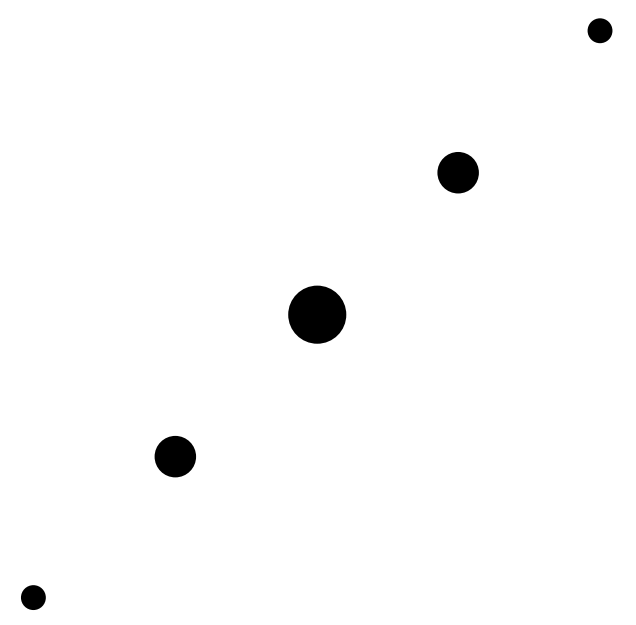
\includegraphics[scale=0.65]{Pictures/45град}
 		\caption{Картина сетки при положении щели под углом $45^\circ$ к вертикали}
 	\end{figure}
 
 	Данные явления происходят потому, что линза осуществляет Фурье-преобразование изображения щели. 
  
  	\newpage
  	
 	\textbf{{\large Вывод:}} в данной работе мы пронаблюдали различные эффекты Фурье-оптики. Также были найдены периоды решеток: $d_1 = (26,2 \pm 0,4)$ мкм, $d_2 = (33,2 \pm 0,7)$ мкм, $d_3 = (69 \pm 3)$ мкм, $d_4 = (141 \pm 6)$ мкм, $d_5 = (185 \pm 7)$ мкм. Мы пронаблюдали эффект мультиплицирования. Было исследовано влияние щелевой диафрагмы на изображение сетки. Все ошибки и погрешности связаны с неточностью измерений и несовершенством их техники.  
  
\end{document}